\documentclass[11pt]{article}

\usepackage[margin=1in]{geometry}
\usepackage{amsmath,amssymb,amsthm}
\usepackage{graphicx}
\usepackage{hyperref}
\hypersetup{hidelinks}

\newtheorem{theorem}{Theorem}
\newtheorem{lemma}[theorem]{Lemma}
\newcommand{\C}{\mathbb C}
\newcommand{\E}{\mathbb E}
\newcommand{\Ran}{\operatorname{Ran}}
\newcommand{\spec}{\sigma}

\title{A nilpotent-drift counterexample to the hypothesis-free\\
$L^1$ Ornstein--Uhlenbeck spectrum extension}
\author{Run \texttt{fa\_banach\_001}, lane 6}
\date{August 13, 2026}

\begin{document}
\maketitle

\begin{abstract}
Kozhan proves that, when the adjoint drift generator $A^*$ has an eigenvalue,
the $L^1$ Ornstein--Uhlenbeck generator has spectrum the closed left half-plane
and every point in the open left half-plane is an eigenvalue.  He asks whether
the theorem extends when $\spec_p(A^*)=\varnothing$.  The literal extension is
false.  Let $S$ be the nilpotent left-shift semigroup on $E=L^2(0,1)$ and take
an injective Hilbert--Schmidt noise operator.  Then $A^*$ has no eigenvalues and
the invariant Gaussian measure is nondegenerate.  Nevertheless, after time one
the Ornstein--Uhlenbeck semigroup is exactly the expectation projection.  On
the mean-zero subspace it is nilpotent, so its generator has entire resolvent;
on constants its generator is zero.  Thus the full $L^1$ generator has
\[
 \spec(L)=\{0\},
\]
not the closed left half-plane.  An earlier paper records the nilpotent-shift
semigroup identity in a $BUC$ norm-continuity discussion; the spectrum inference
and an explicit nondegenerate noise realization are supplied here.
\end{abstract}

\section{Source question}

The source is R. Kozhan, \emph{$L^1$-spectrum of Banach space valued
Ornstein--Uhlenbeck operators}, arXiv:1210.1287 \cite{Source}.  Its main theorem
and hypothesis are:

\begin{center}

\includegraphics[width=0.96\textwidth]{figures/source_theorem_crop.png}
\end{center}

The question appears at the top of the next page:

\begin{center}

\includegraphics[width=0.95\textwidth]{figures/source_question_crop.png}
\end{center}

The standing assumptions include a nondegenerate invariant centered Gaussian
Radon measure $\mu_\infty$.  We satisfy all of them.  The conclusion fails in
the strongest possible spectral way: the only spectral point is zero.

\section{Proof intuition}

The missing hypothesis permits drift semigroups whose generators have empty
spectrum.  The canonical example is the left shift on a finite interval.  It
forgets the entire initial state after one unit of time.  Once the covariance
has accumulated all of its mass, the associated Ornstein--Uhlenbeck transition
therefore also forgets the initial state exactly, not merely asymptotically.

On $L^1(\mu_\infty)$, exact forgetting means that $P(t)$ is the expectation
projection for $t\geq1$.  Removing constants leaves a genuinely nilpotent
$C_0$-semigroup.  The finite Laplace transform of a nilpotent semigroup is a
resolvent at every complex number.  This makes the spectral computation
immediate once the Gaussian measure is verified to be nondegenerate.

\section{The drift and the noise}

Let $E=H=L^2(0,1;\mathbb R)$ and define
\[
 (S(t)f)(r)=
 \begin{cases}
  f(r+t),&r+t\leq1,\\
  0,&r+t>1.
 \end{cases}
\]
This is a strongly continuous contraction semigroup and $S(t)=0$ for
$t\geq1$.

\begin{lemma}\label{lem:adjoint}
If $A$ is the generator of $S$, then $\spec_p(A^*)=\varnothing$.
\end{lemma}

\begin{proof}
On the complexification of $E$,
\[
 Af=f',\qquad
 D(A)=\{f\in H^1(0,1):f(1)=0\}.
\]
Integration by parts gives
\[
 A^*g=-g',\qquad
 D(A^*)=\{g\in H^1(0,1):g(0)=0\}.
\]
If $A^*g=\lambda g$, then $g(r)=ce^{-\lambda r}$.  The boundary condition
$g(0)=0$ forces $c=0$.  This holds for every $\lambda\in\C$.
\end{proof}

Choose an orthonormal basis $(e_n)_{n\geq1}$ of $E$ and define
\[
 Be_n=2^{-n}e_n.
\]
Then $B:H\to E$ is bounded, self-adjoint, injective, nonzero, and
Hilbert--Schmidt.  Put
\[
 Q_t=\int_0^t S(s)B^2S^*(s)\,ds,
 \qquad
 Q_\infty=\int_0^1 S(s)B^2S^*(s)\,ds.                 \tag{1}
\]

\begin{lemma}\label{lem:gaussian}
Each $Q_t$ is the covariance of a centered Gaussian Radon measure $\mu_t$ on
$E$.  The covariance $Q_\infty$ is trace class with dense range, so its
Gaussian measure $\mu_\infty$ is nondegenerate and invariant.  Moreover,
$Q_t=Q_\infty$ for $t\geq1$.
\end{lemma}

\begin{proof}
The operator in (1) is positive, self-adjoint, and
\[
 \operatorname{Tr}Q_t
 =\int_0^{\min(t,1)}\|S(s)B\|_{\mathrm{HS}}^2\,ds
 \leq \|B\|_{\mathrm{HS}}^2<\infty.
\]
Thus it is a Gaussian Radon covariance.  For $x\neq0$,
\[
 \langle Q_\infty x,x\rangle
 =\int_0^1\|B S^*(s)x\|^2\,ds>0.
\]
Indeed, the continuous integrand is strictly positive at $s=0$ because $B$
is injective.  Hence $Q_\infty$ is injective; since it is self-adjoint,
$\overline{\Ran Q_\infty}=E$.  This is exactly nondegeneracy of the centered
Gaussian measure.

The covariance identity
\[
 Q_\infty=Q_t+S(t)Q_\infty S^*(t)
\]
follows by splitting the integral and using the semigroup property, and proves
invariance.  Finally, $S(s)=0$ for $s\geq1$, so (1) gives
$Q_t=Q_\infty$ for every $t\geq1$.
\end{proof}

\section{Exact computation of the \texorpdfstring{$L^1$}{L1} spectrum}

Let $(P(t))_{t\geq0}$ be the Ornstein--Uhlenbeck semigroup on
$L^1(E,\mu_\infty)$ and let $L$ be its generator.

\begin{theorem}\label{thm:counterexample}
For the drift and noise above,
\[
 \spec_p(A^*)=\varnothing,
 \qquad
 \spec(L)=\{0\}.
\]
In particular, the conclusion of source Theorem 1.1 does not extend to all
cases with empty point spectrum of $A^*$.
\end{theorem}

\begin{proof}
The first assertion is Lemma~\ref{lem:adjoint}.  For $t\geq1$ the Mehler
formula, Lemma~\ref{lem:gaussian}, and $S(t)=0$ give
\[
 P(t)f(x)=\int_E f(y)\,d\mu_\infty(y)=:\Pi f.          \tag{2}
\]
This holds first for bounded Borel functions and hence for the unique
contraction extension to $L^1(E,\mu_\infty)$.

Use the bounded invariant decomposition
\[
 L^1(E,\mu_\infty)
 =\C\mathbf1\oplus X_0,
 \qquad X_0:=\ker\Pi.
\]
On constants $P(t)$ is the identity, so the generator is zero.  The restricted
semigroup $P_0(t):=P(t)|_{X_0}$ satisfies $P_0(t)=0$ for $t\geq1$ by (2).
Let $L_0$ be its generator.  For arbitrary $\lambda\in\C$ define the bounded
operator
\[
 R_\lambda f:=\int_0^1e^{-\lambda t}P_0(t)f\,dt.
\]
The standard semigroup differentiation calculation, whose endpoint term is
$e^{-\lambda}P_0(1)=0$, gives
\[
 (\lambda-L_0)R_\lambda f=f\quad(f\in X_0),
 \qquad
 R_\lambda(\lambda-L_0)g=g\quad(g\in D(L_0)).
\]
Thus every $\lambda\in\C$ belongs to the resolvent set of $L_0$.

For $\lambda\neq0$, the inverse of $\lambda-L$ on the displayed direct sum is
\[
 (\lambda-L)^{-1}(c\mathbf1+g)
 =\frac c\lambda\mathbf1+R_\lambda g.
\]
Hence $\C\setminus\{0\}\subseteq\rho(L)$.  On the other hand,
$L\mathbf1=0$, so zero is an eigenvalue.  Therefore $\spec(L)=\{0\}$.
\end{proof}

\section{Prior overlap, limitations, and novelty audit}

Van Neerven and Priola already used the same nilpotent shift in a discussion of
norm discontinuity on $BUC$ and observed $S(t)=0$, $\mu_t=\mu_1$, and
$P(t)=P(s)$ for $t,s\geq1$ \cite[Example 2.9]{Prior}:

\begin{center}
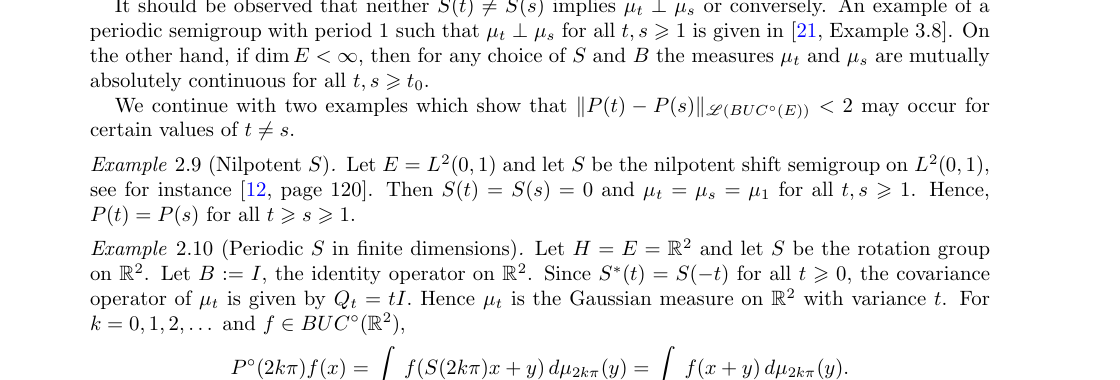
\includegraphics[width=0.96\textwidth]{figures/prior_nilpotent_crop.png}
\end{center}

That example is decisive supporting evidence rather than a later solution of
the 2012 question: it predates the question and does not state the $L^1$
generator spectrum.  The present packet makes the implication explicit,
chooses an injective Hilbert--Schmidt noise so every standing Gaussian and
nondegeneracy assumption is verified, and supplies the entire-resolvent
calculation.

The counterexample exploits $\spec(A)=\varnothing$, as is possible for a
nilpotent $C_0$-semigroup generator.  It does not settle the sharpened question
in which one additionally assumes $\spec(A)\neq\varnothing$ while retaining
$\spec_p(A^*)=\varnothing$.

A bounded search on August 13, 2026 checked all four lightweight run indexes,
the exact title/id, the exact open-question phrase, and nilpotent-shift OU
spectrum keywords.  It found the source, standard finite-dimensional results,
surveys, and the prior example above, but no paper stating this $L^1$ spectral
counterexample.  The result is recommended for expert review as a likely valid
full negative answer to the question as literally worded, with deliberately
limited novelty claims.

\begin{thebibliography}{9}
\bibitem{Source}
R. Kozhan,
\emph{$L^1$-spectrum of Banach space valued Ornstein--Uhlenbeck operators},
Semigroup Forum 78 (2009), 547--553; arXiv:1210.1287.

\bibitem{Prior}
J. M. A. M. van Neerven and E. Priola,
\emph{Norm discontinuity and spectral properties of Ornstein--Uhlenbeck
semigroups},
J. Evol. Equ. 5 (2005), 473--488.
\end{thebibliography}

\end{document}
